\documentclass[aspectratio=169]{beamer}

\usepackage[utf8]{inputenc}
\usepackage{graphicx}
\usepackage{url}
\usepackage{listings}
\usepackage{xcolor}
\usepackage{minted}

\usetheme{metropolis}

\definecolor{codegreen}{rgb}{0,0.6,0}
\definecolor{codegray}{rgb}{0.5,0.5,0.5}
\definecolor{codepurple}{rgb}{0.58,0,0.82}
\definecolor{backcolour}{rgb}{0.95,0.95,0.92}

\lstdefinestyle{mystyle}{
    backgroundcolor=\color{backcolour},
    commentstyle=\color{codegreen},
    keywordstyle=\color{magenta},
    numberstyle=\tiny\color{codegray},
    stringstyle=\color{codepurple},
    basicstyle=\ttfamily\footnotesize,
    breakatwhitespace=false,
    breaklines=true,
    captionpos=b,
    keepspaces=true,
    numbers=left,
    numbersep=5pt,
    showspaces=false,
    showstringspaces=false,
    showtabs=false,
    tabsize=2
}

\lstset{style=mystyle}

\title{Zig Workshop}
\author{Joachim Schmidt}
\date{15. Oktober 2021}

\begin{document}

%\frame{\titlepage}

\begin{frame}{}
  \begin{figure}
    \centering
    \includegraphics[width=\textwidth]{zig-logo-dark.png}
    \caption{\cite{logo}}
    \label{fig:logo}
  \end{figure}
\end{frame}

\begin{frame}{}
  \tableofcontents
\end{frame}

\section{Einführung}

\begin{frame}{Die Zig Programmiersprache}
  \begin{itemize}
  \item imperativ
  \item statisch typisiert
  \item low-level / manuelles Speichermanagement
  \item Ausführung von Code zur Kompilierzeit
  \end{itemize}
\end{frame}

\begin{frame}{Hello World}
  \inputminted[linenos]{zig}{examples/hello.zig}
\end{frame}

\section{Überblick}

\begin{frame}{Primitive Typen}
  \inputminted[linenos]{zig}{examples/primitive_types.zig}
\end{frame}

\begin{frame}{Deklarationen}
  \inputminted[linenos]{zig}{examples/decls.zig}
\end{frame}

\begin{frame}{Funktionen}
  \inputminted[linenos]{zig}{examples/functions.zig}
\end{frame}

\begin{frame}{Arrays}
  Wenn \mint{zig}|T| ein Typ ist, dann ist \mint{zig}|[10]T| ein Array der Länge 10 von diesem Typ
  \inputminted[linenos]{zig}{examples/arrays.zig}
\end{frame}

\begin{frame}{Pointer}
  \inputminted[linenos]{zig}{examples/pointer.zig}
\end{frame}

\begin{frame}{Slices}
  \inputminted[linenos]{zig}{examples/slices.zig}
\end{frame}

\begin{frame}{Structs}
  \inputminted[linenos]{zig}{examples/structs.zig}
\end{frame}

\begin{frame}{if}
  \inputminted[linenos]{zig}{examples/if.zig}
\end{frame}

\begin{frame}{switch}
  \inputminted[linenos]{zig}{examples/switch.zig}
\end{frame}

\begin{frame}{for}
  \inputminted[linenos]{zig}{examples/for.zig}
\end{frame}

\begin{frame}{while}
  \inputminted[linenos]{zig}{examples/while.zig}
\end{frame}

\section{Besonderheiten}

\begin{frame}{Besonderheiten}
  \begin{itemize}
  \item manuelles Speichermanagement
  \item Ausführung von Code zur Kompilierzeit
  \item Integration mit C
  \end{itemize}
\end{frame}

\begin{frame}{Manuelles Speichermanagement...}
  \inputminted[linenos]{zig}{examples/manual.zig}
\end{frame}

\begin{frame}[fragile]{...ist riskant}
\begin{verbatim}
Segmentation fault at address 0x7f2e08661000
./manual.zig:12:40: 0x22b9f7 in main (manual)
    std.debug.warn("{}\n", .{list.items[0]});
                                       ^
\end{verbatim}
\end{frame}

\begin{frame}{Ausführung von Code zur Kompilierzeit}
  \inputminted[linenos, fontsize=\small]{zig}{examples/comptime.zig}
\end{frame}

\begin{frame}{Integration mit C}
  \inputminted[linenos, fontsize=\small]{zig}{examples/c_integration.zig}
\end{frame}

\section{Weiterführendes}

\begin{frame}{Links}
  \begin{itemize}
  \item Quellcode: \url{https://github.com/joachimschmidt557/zig-workshop-ophase2021}
  \item Homepage: \url{https://ziglang.org}
  \item Github: \url{https://github.com/ziglang/zig}
  \item Ziglearn: \url{https://ziglearn.org}
  \item Ziglings: \url{https://github.com/ratfactor/ziglings}
  \item Zig Showtime: \url{https://zig.show}
  \end{itemize}
\end{frame}

\begin{frame}{Video: The Road to Zig 1.0}
  \begin{figure}
    \centering
    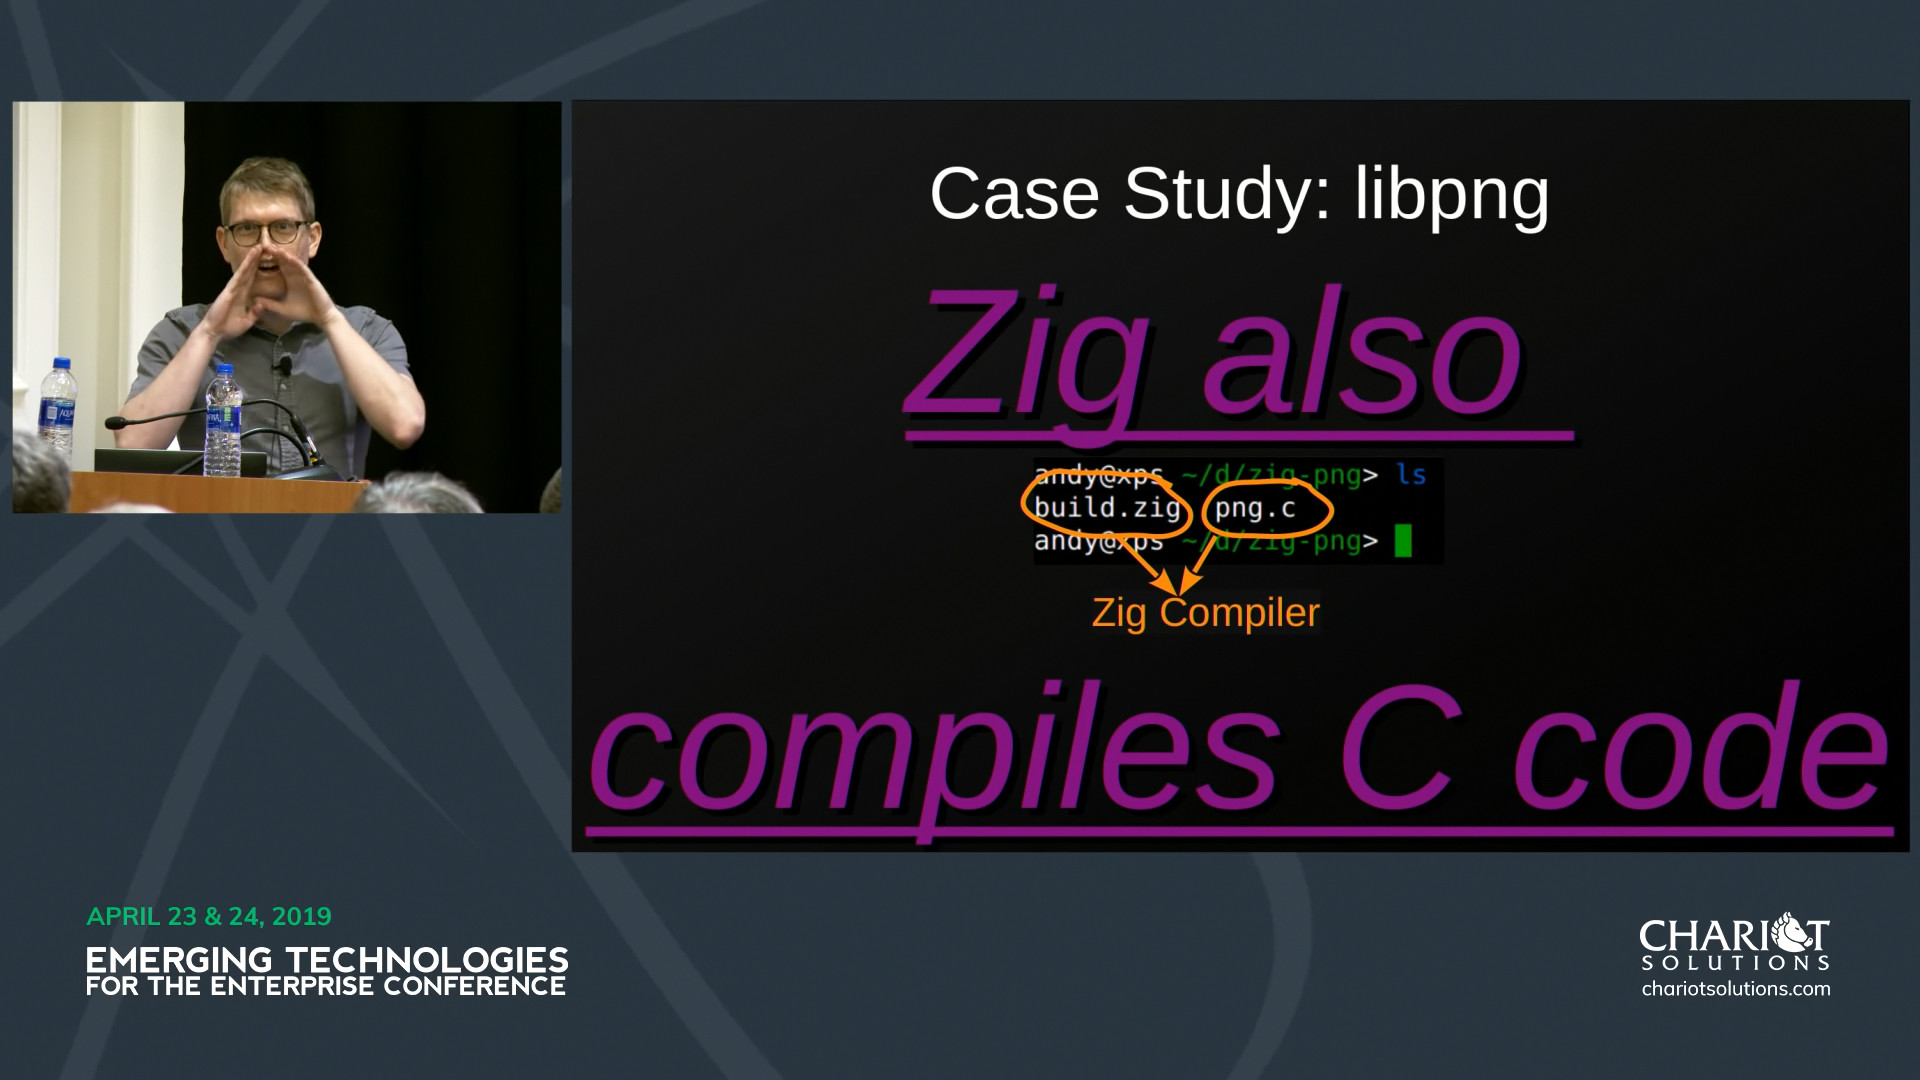
\includegraphics[height=0.8\textheight]{img/mpv-shot0002.jpg}
    \caption{\url{https://youtu.be/Gv2I7qTux7g}}
    \label{fig:road-zig-1-0}
  \end{figure}
\end{frame}

\begin{frame}{Video: Implementing an ARM backend for stage2}
  \begin{figure}
    \centering
    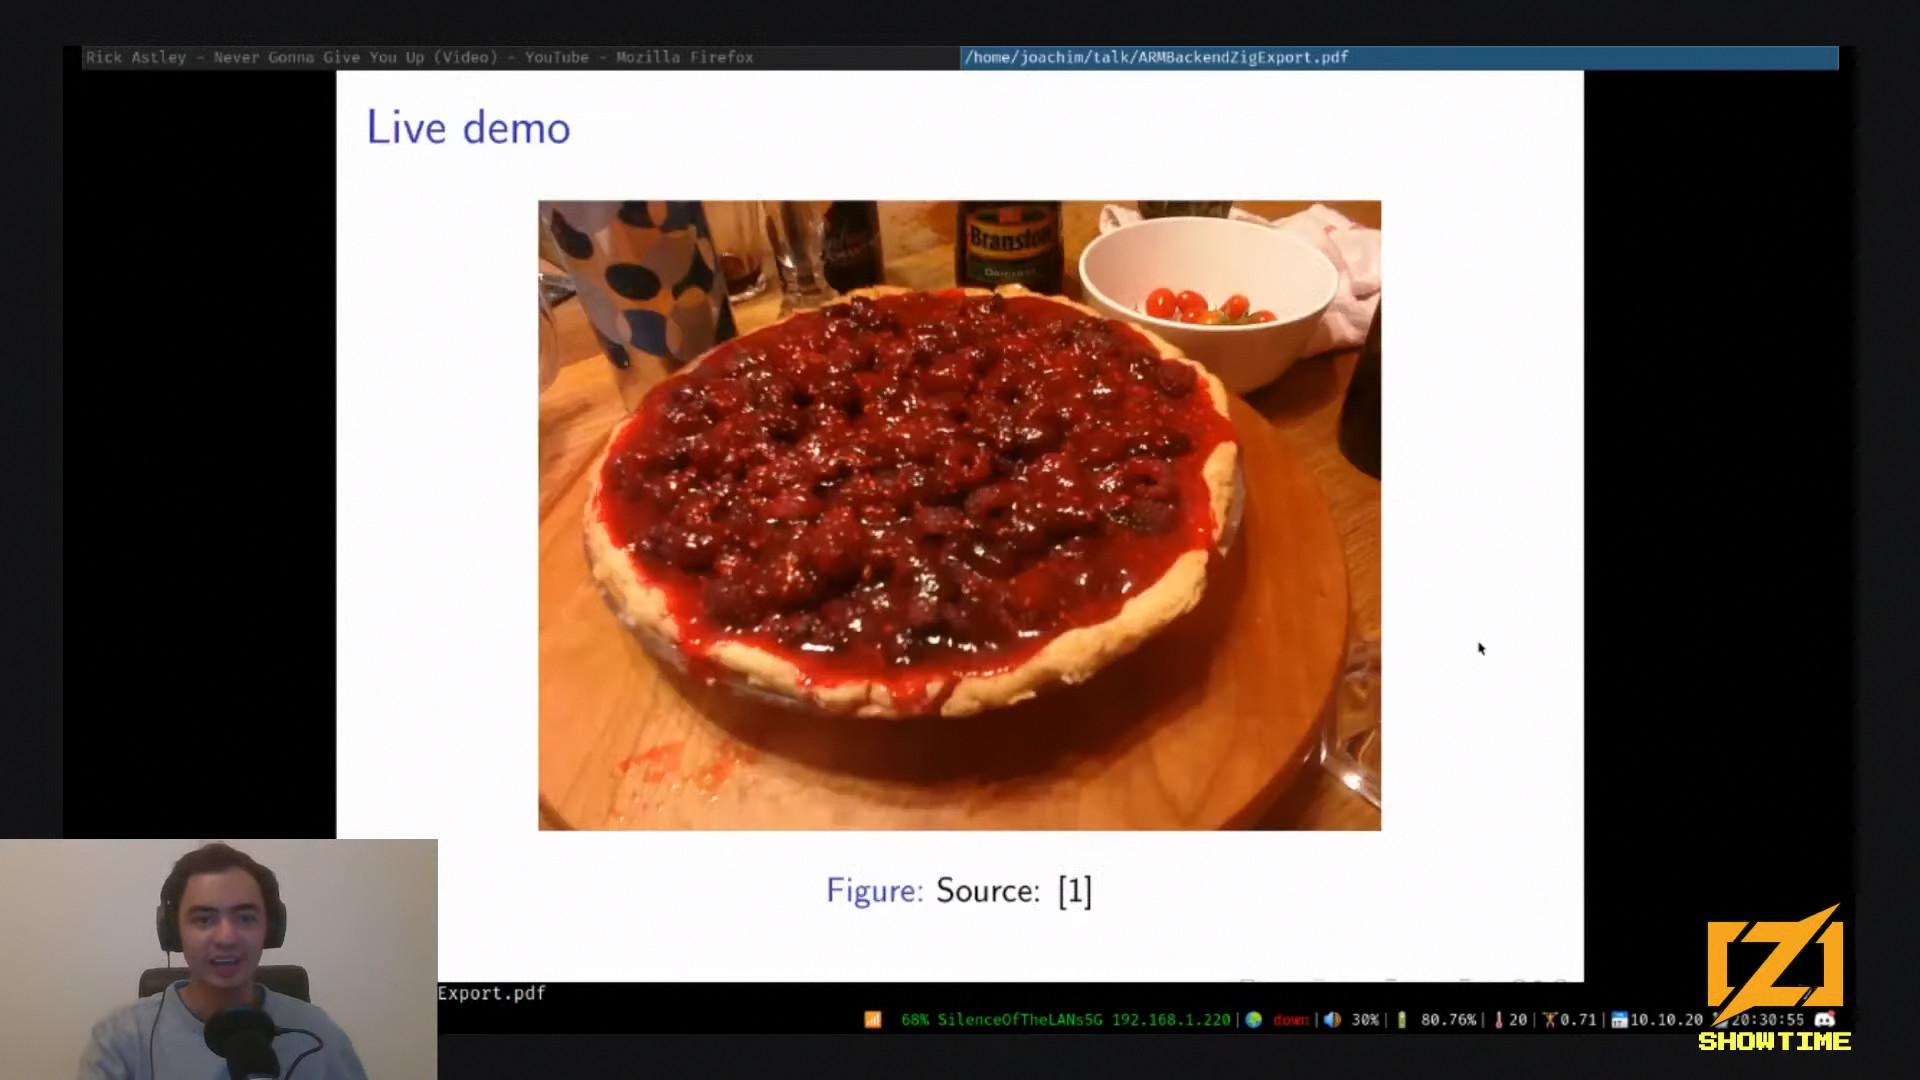
\includegraphics[height=0.8\textheight]{img/mpv-shot0001.jpg}
    \caption{\url{https://youtu.be/qNKGaePky04}}
    \label{fig:arm-backend}
  \end{figure}
\end{frame}

\section{Live Q\&A und Live Coding}

\begin{frame}{Live Q\&A und Live Coding}
  \begin{figure}
    \centering
    \includegraphics[height=0.8\textheight]{zero.png}
    \caption{Zero, eines der Zig Maskottchen \cite{zero}}
    \label{fig:zero}
  \end{figure}
\end{frame}

\begin{frame}{Quellen}
  \begin{thebibliography}{}
  \bibitem{logo}
    \url{https://github.com/ziglang/logo/raw/master/zig-logo-dark.svg}

  \bibitem{zero}
    \url{https://github.com/ziglang/logo/raw/master/zero.svg}

  \end{thebibliography}
\end{frame}

\end{document}
